\chapter{Analysis of the Neural Engineering Framework}
\label{chapt:analysis}

In this chapter, we provide a thorough examination of the Neural Engineering Framework~\citep[NEF;][]{eliasmith2003a} that is not currently published elsewhere.
The goals are two-fold: (1)~explore the consequences of its computational principles at a theoretical level, and in doing so challenge some common myths that have become associated with the NEF since its inception, and (2)~assess its suitability as a framework for deploying SNNs on neuromorphic hardware by proving its correctness, scalability, completeness, robustness, and extensibility.\footnote{%
To help delineate separate considerations, some sub-sections are significantly shorter than others.
}
% This involves a proof of equation~\ref{eq:rate-approximation} thatextends and improves the discussion of \citet[][pp.~132--136]{eliasmith2003a} to provide a sufficient criteria for the correctness of the first two principles of the NEF at the level of individual spikes.
% The correctness of the third principle is proven in \citet[][pp.~221--225]{eliasmith2003a} and is extended by various proofs in section~\ref{sec:synaptic-extensions}.

\section{Computational Sub-Principles}
\label{sec:sub-principles}

In this section, we focus primarily on the third principle of the NEF, and elucidate some high-level observations, or ``sub-principles,'' that follow from its adoption.
In doing so, we expose some important insights, including the effects of structuring deep RNNs, a framework to understand the roles of dynamical primitives, the observation of chaos in simple NEF networks, its strategy for neural encoding, and a relationship between the energy of synaptic events and signal bandwidth.

\subsection{Reducibility to a single layer}

In section~\ref{sec:nef}, we focused primarily on a single recurrently connected population of neurons.
However, any multi-layer NEF network, where each layer may be recurrent, with feed-forward connections and feedback connections optionally included between any two layers -- may be rewritten as a single recurrently connected population.
Indeed, even for models as complex as Spaun~\citep{eliasmith2012, choo2018}, the Nengo builder strips away the model specification, and leaves only channels that transmit spikes, and transfer functions that operate on these spikes~\citep{bekolay2014, gosmann2017automatic}.
The topology of the network reflects spatial and organizational structure (e.g.,~hierarchies), which may be used to constrain and inform the design of biologically-grounded models and to aid in understanding function.
The mechanisms underneath are mere signals and operators, all coupled to one another to implement some dynamical system.

To examine some of the consequences of this observation, we assume without loss of generality that there are $m$ layers, and that each layer uses $n$ neurons to represent a $q$-dimensional state-vector.
The procedure for rewriting the network is as follows:
\begin{enumerate}
\item Stack all of the populations together into a single layer that consists of $nm$ neurons. 
\item Stack all of the state-vectors together into one vector, $\V{x}(t) \in \mathbb{R}^{qm}$, to represent the global state-space.
\item Construct the encoding matrix, $E \in \mathbb{R}^{nm \times qm}$, by inserting the encoding matrix from the $i^\text{th}$ population into the $(i\text{,} i)^\text{th}$ block, such that $E$ is in block-diagonal form (note: there are $m \times m$ blocks and each is $n \times q$).
\item Construct the decoding matrix, $D^\V{f} \in \mathbb{R}^{nm \times qm}$, by inserting each decoding matrix $D^{\V{f}_{i\text{,}j}}$ into the $(i\text{,} j)^\text{th}$ block, where $\V{f}_{i\text{,}j}$ is the function computed between the $i^\text{th}$ presynaptic population and the $j^\text{th}$ postsynaptic population.
\end{enumerate}
Then Principles~1--3 apply in the same way to this single population, while being functionally equivalent to the original network.

This reveals that the problem of constructing and training arbitrary network topologies may be reduced to the special case of a single layer.
Conversely, we do not lose any computational power by limiting our focus to a single layer.
However, the encoding matrix is extremely sparse with $(m - 1) / m$ percent of its coefficients set to zero.
Likewise, the block-structure of the decoding matrix is isomorphic to the graph structure of the original network.

This characterizes the functional role of network structure as: partitioning the global state-space into a union of state-vectors with a range of time-constants, sparsifying its encoders, and rearranging the decoders into a block-structure that mirrors the interactions between subspaces.
In terms of computation, the network structure dramatically reduces the time and memory requirements that would otherwise be needed for a full-rank $nm \times nm$ matrix multiplication.
In terms of training, the challenges involved in globally optimizing an RNN may be viewed under the lens of identifying relatively low-dimensional subspaces acting along various time-scales and their interactions with one another.

\subsection{Heterogeneity of dynamical primitives}

We make the observation that neurons~(equation~\ref{eq:lif-model}), synapses~(equation~\ref{eq:lowpass-impulse}), and even the functional behaviour of entire recurrent networks~(equations~\ref{eq:discrete-dynamical-system} and~\ref{eq:lti}), are all described in terms of differential equations.
These dynamical systems, each of which can be thought of as a \emph{primitive} for use in some larger computation, all have distinct filtering properties, linear and nonlinear transfer functions, and internal states that evolve over time in response to some input in order to produce some output.

A central insight from deep learning is that a variety\footnote{%
The variety of nonlinear responses comes from the distribution of weights and biases, analogous to the heterogeneity obtained in equation~\ref{eq:encoding} via encoding vectors, gains, and biases.}
of static nonlinear functions, when structurally composed, enhance the \emph{spatial complexity} of network function.
An analogous insight in the above context is that a variety of transfer functions, when temporally composed, enhance the \emph{temporal complexity} of network function.
In particular, the time-constants of synaptic currents, membrane leakages, and recurrent network dynamics -- all act along different time-scales.
In effect, NEF networks compose rich temporal functions by leveraging dynamical primitives that are heterogeneous in time.
A compelling example is provided in section~\ref{sec:delay-lstm}, where we apply BPTT to a deep recurrent NEF network to predict a chaotic time-series.

\subsection{Duality of macroscopic and microscopic dynamics}

As a corollary to the previous observation,
once all primitive operations are expressed in the same language (i.e.,~differential equations), they become both \emph{composable} and \emph{interchangeable}.
To the point of interchangeability, one can implement a lowpass filter by using a single synapse, or by training a population to emulate the same dynamical system via Principle~3.\footnote{%
As inconsequential as this point might sound, a potent example is when one student, who had been working with Nengo for many years, used a network containing hundreds of neurons to implement the same computation as a single alpha synapse. This was due to not having them described in the same language.}
To the point of composability, one can substitute the transfer function of a single synapse with that of an entire recurrent network.

We illustrate both points with a specific example by considering the following architecture:
$$A \rightarrow (B \rightarrow B) \rightarrow A \text{,}$$
where $A$ and $B$ are separate neural ensembles and ``$\rightarrow$'' denotes a synaptic weight matrix.
That is, $B$ is locally-recurrent, and $A$ is globally-recurrent via the outer loop through $B$.
We may encapsulate $H = B \rightarrow B$ as a dynamical primitive, and then re-interpret the whole system as:
$$A \rightarrow_H A \text{,}$$
where ``$\rightarrow_H$'' denotes some weight matrix where the \emph{synapse} model has been replaced by $H$ --
akin to a ``virtual'' synapse, whose dynamics are implemented by $B$ under the hood.
This is simply a mathematical ``trick,'' but the practical consequence is that we may use the same theory and the same tools to understand the composition and substitution of these systems.
This is made possible since we employ a common language and framework for describing and leveraging dynamical systems.

In section~\ref{sec:linear-extensions}, this idea forms the core idea for our proofs that extend Principle~3.
In section~\ref{sec:pure_delay}, we demonstrate a method of systematically harnessing miniature delays in axonal spike-transmission to improve the accuracy of longer network-level delays.

\subsection{Unpredictability, chaos, and strange attractors}
\label{sec:chaos}

An apparent misconception associated with NEF networks is that we already ``understand'' the computations being engineered into the network, and therefore have nothing to learn from such simulations.
But just because a network's function can be written down using equations, does not mean that its effects are fully understood ahead of time.
For example, the NEF has been used to construct chaotic systems, such as the Lorenz strange attractor~\citep{eliasmith2005b}.
This \emph{deterministic} system is fully described by a three-dimensional nonlinear dynamical system.
However, due to the nature of such chaotic systems, arbitrarily small perturbations in state-space diverge exponentially over time up to the diameter of the attractor~\citep[][pp.~328--330]{strogatz2000nonlinear}.
This leads to a fundamental inability to predict the trajectory of any physical instantiation of the system; the time-horizon that can be predicted, within some given tolerance, scales only logarithmically with the precision of the observer.

More to the point, this accusation is theoretically equivalent to suggesting the same of any algorithm or computer program for that matter.
Even though \emph{any} computer program can be written down using a finite set of symbolic expressions, and realized as a discrete sequence of steps that dynamically evolve a set of registers---such as the machine of \citet{turing1938computable}---does not mean that we know what that program will compute ahead of time on any given input.
The assertion that the behaviour of certain programs are in essence ``unpredictable'' corresponds with the notion of \emph{undecidability} in formal theories of computation; informally, most non-trivial programs need to be run in order to see what they will do with their inputs.

This discussion extends to dynamical systems, where chaos and undecidability are also interwoven~\citep{moore1991generalized}.
For example, suppose we take the linear time-invariant~(LTI) system of equation~\ref{eq:lti} and then include saturation within each of the state-variables (such that their absolute magnitudes cannot exceed one).
Surprisingly, this is a sufficient route to chaos.
The inclusion of this single nonlinearity spawns attractors with properties that are undecidable~\citep{blondel2001stability}; basic questions about the system's response cannot be resolved in a finite number of steps~\citep{bennett1990undecidable}.
This example is of special interest to us since the LIF neuron (equation~\ref{eq:lif-model}) exhibits a similar saturation effect, namely $r(\V{v}) \le \tau_\text{ref}^{-1}$, where the upper-bound is approached as $\V{x}(t) \in \mathbb{R}^q$ extends beyond the representational range established by the encoding parameters selected by Principle~1.
It follows that even the most basic spiking instantiation of Principle~3 must, in general, be simulated in order to determine its behaviour whenever the input signal drives the state-space outside the range of neural representation.
Notably, this saturation effect is exploited to overload working memory with sequential items in the Spaun model~\citep{eliasmith2012}, which suggests that the model behaviour is chaotic at multiple levels of analysis.

\fig{chaotic-integrator}{1}{Chaos in a simple Neural Engineering Framework network.}{
      An autonomous scalar integrator---the simplest possible recurrent SNN, built using the NEF---exhibiting chaotic neural dynamics.
      (Left)~Two deterministic simulations of the exact same network.
          One is initialized to $x_1(0) = 0$, and the other to $x_2(0) = \numprint{e-15}$.
          Both simulations fall into the same apparent strange attractor, close to zero.
      (Right)~Plotting the difference in representational states~($\Delta$) and neural states~($\delta$) on a logarithmic scale.
          The neural states diverge exponentially quickly---leaping 30 orders of magnitude in 3 seconds---according to $\| \delta(t) \| \approx \bigoh{e^{\lambda t}}$.
          The representational difference $\Delta$ is essentially zero until $\delta$ hits the diameter of the attractor.
          It is physically impossible to predict the future state of this system beyond a time-scale of $\bigoh{\lambda^{-1}} \approx 0.1$~seconds (see text for details).
}

Perhaps even more surprisingly, one does not need to invoke any saturation to observe chaos, at the level of individual spiking neurons, in NEF networks implementing linear dynamics.
For example, consider the one-dimensional, autonomous (i.e.,~no input), integrator:
$$\dot{x}(t) = 0 \text{,}$$
implemented as an SNN using Principle~3 of the NEF ($A = B = D = 0$, $C = 1$).
This is perhaps the simplest recurrent network that one can imagine; a line attractor without input, that is to hold its initial state indefinitely.
Nevertheless, as shown in Figure~\ref{fig:chaotic-integrator}, the neural states display the tell-tale signs of a strange attractor~\citep[cf.~][Figure~9.3.5]{strogatz2000nonlinear}.
Specifically, let $\V{v}_1(t), \V{v}_2(t) \in \mathbb{R}^n$ be two voltage vectors (see equation~\ref{eq:lif-model}) from two separate, but deterministic simulations, of the \emph{exact} same network ($n = 10$, $\tau = 5$\,ms, $\dt{} = 0.1$\,ms, down-sampled every $20$\,ms).
The first simulation is initialized to the default of $x_1(0) = 0$, while the second is initialized to $x_2(0) = \numprint{e-15}$.
% Both fall into the same attractor basins, decoding an approximation of $0$, that persists indefinitely through recurrent feedback.
Now let:
\begin{align*}
\Delta(t) &= x_1(t) - x_2(t) \\
\delta(t) &= \V{v}_1(t) - \V{v}_2(t) \text{,}
\end{align*}
be the difference in representational state and neural state, respectively.
We find that $\Delta$ remains bounded above by the accuracy of neural representation, as expected.
However, $\delta$ diverges exponentially over time, consistent with the neural states being within a strange attractor (the Lyapunov exponent $\lambda \approx 8.9$\,s${}^{-1}$ gives the exponential rate of divergence); the voltage vectors are tracing out a fractal manifold embedded within an $n$-dimensional space that cannot be predicted beyond a time-horizon on the order of $\bigoh{\lambda^{-1}} \approx 0.1$\,s.
Despite this, the NEF is capable of taming the chaos at the neural level and providing a robust estimate at the population level, due to the correspondence between each apparent strange attractor and a stable point in representational space~\citep[][p.~237]{eliasmith2003a}.
In section~\ref{sec:nef-robustness}, we remark that this leads to the NEF being robust to a distinctly different type of error.

At a high level, the NEF may be used to implement arbitrary algorithms encoded as dynamical systems (see section~\ref{sec:nef-turing}), which implies that it is not exempt from computability theory. 
Networks can perform interesting tasks via algorithmic manipulations of inputs and states~\citep{choo2018}.
Then, as is the case for any Turing machine, the network must in general be simulated to carry out the computations of said algorithm.
At the same time, the NEF provides a framework---akin to having a programming language for some model of computation---to understand the dynamical transformations being performed, examine relationships between structure and function, relate these functions to neurobiological systems, and compile them onto neuromorphic hardware.

\iffalse
\subsection{Continuous-Time and Discrete-Time}

The idea that both continuous-time and discrete-time dynamics play important roles at different time-scales, both in terms of the dominant dynamics and in terms of the desired computation.
It is also important to consider both for neuromorphic hardware.
\fi

\subsection{Coding by postsynaptic currents}
\label{sec:psc-coding}

A long-standing debate in neuroscience has traditionally revolved around the question of whether biological neurons transmit information using a ``rate code'' in which the information is encoded by the firing rates of individual neurons~\citep{adrian1928basis}, or a ``spike-timing code'' in which information is encoded by the precise temporal patterns of spike trains~\citep{rieke1999spikes} or likewise their temporal order in relation to one another~\citep{thorpe1998rank}.
However, there is historically little consensus between neuroscientists as to what exactly constitutes a rate code~\citep[][pp.~89--91]{eliasmith2003a}.

\citet{gerstner1999spiking} reviews at least three different ways to define a rate code, and notes that in many important ways they are consistent with that of a timing-based code.
\citet{fairhall2001efficiency} models the adaptive dynamics of neurons in the fly visual system and concludes that principles of its code depend on the time-scale of interest.
\citet{brette2015philosophy} argues that which code the brain uses is irrelevant, and that we ought to instead consider questions that address the causal role of neural activity.
\citet{eliasmith2003a} likewise proposes that we should focus on the physical instantiation, and functional consequences therein, of any given approach to neural coding, rather than resorting to semantic labels that are ultimately irrelevant. 

\fig{spike-time-coding}{1}{Spike-time coding in the Neural Engineering Framework.}{
      Demonstrating the irrelevance of identifying a ``spike-time code'' versus a ``rate code'' in the context of a standard NEF-optimized network.
      We define this as a ``postsynaptic current code'' instead.
      (Left)~An ensemble of LIF neurons are trained to oscillate at approximately $3.5$\,Hz.
      (Right)~Spike rasters of \numprint{50} randomly selected neurons, ordered by their encoding vector's polar angle.
      Each neuron spikes only $0$, $1$, or $2$ times per oscillation, and at a precise moment in time---on the order of milliseconds (see inset)---before remaining silent for another couple hundred milliseconds.
      Thus, the precise spike-timing of each individual neuron reliably conveys information about the state-space of the oscillation, despite never explicitly incorporating such a requirement about timing into the training procedure.
}

Nevertheless, many have mislabelled the NEF as employing a rate-coding scheme [personal communication], including \citet{lagorce2015stick} and~\citet{frady2019robust} for two recent examples -- we refer to these two below, to illustrate why this accusation constitutes a damaging use of semantics.
% On one hand, we understand that this is due to the way in which the optimization procedure is most often simplified using equation~\ref{eq:rate-approximation}.
Specifically, this mischaracterization has lead to the misapplication of many criticisms~\citep{gautrais1998rate} that stem from the original proposal of \citet{adrian1928basis}, namely the need to average spike rates over long windows of time.
We find this important to clarify because it leads to imprudent conclusions or ``myths'' about the NEF such as those claimed by \citet{lagorce2015stick} and \citet{frady2019robust}:
\begin{enumerate}
\item The NEF does not exhibit precise sequences of action-potentials.
\item The NEF does not support high-speed neural computation.
\item The NEF does not display rhythmic activity.
\item The NEF requires very large numbers of neurons to compute simple functions.
\end{enumerate}
We now challenge each claim in turn.
For the first three, we refer to the same simulation depicted in Figure~\ref{fig:spike-time-coding}.
This simulation applies the NEF, as described in section~\ref{sec:nef}, to the case of an autonomous two-dimensional oscillator ($n = \numprint{5000}$, $\tau = 0.1$\,s, $\dt{} = 1$\,ms).
The encoding parameters are randomly tiled across the two-dimensional state-space such that each neuron only responds to 25\% of the state's projection onto its encoder (i.e.,~uniform $[0.5, 1)$ intercepts), and each neuron \emph{would} fire at a rate of $20$--$40$\,Hz if encoding a constant state with maximal similarity to its encoder.
As we explain, the firing statistics are not at all characterized by $20$--$40$\,Hz spike-trains.
We omit the first $1.2$ seconds of simulation to avoid initial transients.

\paragraph{1. The NEF can exhibit repeatedly precise sequences of action-potentials.}

See Figure~\ref{fig:spike-time-coding}~inset.
When comparing the spike-trains between two separate oscillations at the same phase, not only is the order of spiking consistent, as in rank order coding~\citep{thorpe1998rank}, but also the precise spike-timing ($\pm$ a couple milliseconds).

\paragraph{2. The NEF readily supports high-speed neural information processing.}

In our example, neurons respond quickly to encode the rapidly-fluctuating oscillatory state, and do so without any system-level ``delay'' or undesired filtering.\footnote{%
The postsynaptic filters are leveraged to participate in the required computation (see Principle~3; section~\ref{sec:principle3}).
There is no unwanted phase-shift.
}
As will be explained in section~\ref{sec:spike-coding}, the precision of a feed-forward network scales as $\bigoh{\tau \sqrt{n}}$.
Thus, one is free to set the synaptic time-constant arbitrarily small, so long as the number of neurons are increased in proportion.
We have verified this both theoretically and numerically in section~\ref{sec:poisson-spiking}.
This enables arbitrarily fast transmission of information throughout the network assuming the criteria of Theorem~\ref{thm:correctness} is met (also see Figure~\ref{fig:poisson-frequency-scaling}).
Yet, even when constrained to longer time-constants, section~\ref{sec:deep-delay-networks} demonstrates a novel deep NEF network that is capable of \emph{instantaneously} propagating low-frequency stimuli through 8 layers of synaptic filters ($\tau = 0.1$\,s).

\paragraph{3. The NEF examples that invoke Principle~3 all display rhythmic activity.}

The NEF was designed as a toolkit for modelling dynamic rhythmic activity~\citep{eliasmith1999developing} such as the central pattern generator driving lamprey locomotion~\citep{eliasmith2000b}.
Indeed, Figure~\ref{fig:spike-time-coding} clearly displays rhythmic activity at both the population level~(see left) and the activity level~(see right).
The properties of these rhythms can be understood as arising from the dynamics of the postsynaptic currents, in response to the neural encoding of the state-vector governed by some underlying set of differential equations.

\paragraph{4. The NEF can compute difficult functions with any number of neurons.}

See Figure~\ref{fig:chaotic-integrator} for an example of ten spiking LIF neurons implementing a line attractor ($\tau = 5$\,ms), or section~\ref{sec:delay-lstm} for a six neuron cell that outperforms LSTM cells.
No matter how complex the function, the mandate of the NEF is to leverage its neuron models as a basis for that function. 
Sometimes this can be done with sufficient accuracy using a single neuron, and in other cases one might need a few million or even more.
In general, the feed-forward precision scales as $\bigoh{\tau \sqrt{n}}$ while the dynamical precision scales as $\bigoh{\theta \sqrt{n}}$, where $\theta$ is the time-constant of the dynamical system (under fairly weak assumptions; see section~\ref{sec:spike-coding}).
But one cannot consider the questions of resource usage and functional precision within a vacuum.
One must resolve such questions with respect to the device-level models of the physical hardware implementation as well as the intended target application.
Some advances in this direction are underway~\citep{schwemmer2015constructing, thalmeier2016learning}.
But many other considerations such as weight factorization, mechanistic constraints, and the energy consumed by different synaptic or neural operations, may all play a role.
If one is interested in constructing functioning dynamical SNNs using neuromorphic hardware, we suggest that one considers all such factors in the context of the target application before labelling an approach as being unequivocally inferior.

The confusion surrounding rate coding in the NEF has essentially risen from the adoption of equation~\ref{eq:rate-approximation}.
However, as we have said, this merely reformulates the optimization procedure to be more efficient, without sacrificing correctness as proven in section~\ref{sec:spike-coding}.
We remark that, in Figure~\ref{fig:spike-time-coding}, the firing statistics are completely unlike their rate model counterparts, despite the target postsynaptic currents and overall system dynamics remaining the same.
That is, each neuron only fires at an average rate of $3$\,Hz across the simulation, much slower than the $20$--$40$\,Hz rate that they would fire at for constant inputs.
Likewise, the postsynaptic impulse response that results from a single spike, decays to a factor of $e^{-\frac{10}{3}} \approx 3.5\%$, before \emph{that same} neuron triggers another spike, on average.
In general neither the average rates, inter-spike intervals, nor spike times tell the entire story.

But then how does equation~\ref{eq:rate-approximation} hold if each neuron is not spiking at its intended rate?
Our proposal to resolve this seemingly paradoxical situation is to first establish a new label: ``postsynaptic current code.''
This code does not care about the spike-rates of individual neurons; it is only sensitive to how well the weighted and synaptically-filtered spikes, \emph{when pooled across the entire population}, approximate some desired set of postsynaptic currents~\citep[corresponding to an affine transformation of the required state-vector;][]{tripp2006neural}.
This is summarized by taking the encoding equation~\ref{eq:encoding} and decoding equation~\ref{eq:trans-decode} which fold into the weight equation~\ref{eq:factored-weights} -- and combining them in a similar manner to \citet{stoeckel2018}:
\begin{equation} \label{eq:psc-code}
\alpha_i \left\langle \V{e}_i\text{,}\, \V{x}(t) \right\rangle + \beta_i \approx \sum_{j=1}^n \sum_m \omega_{ij} h \left( t - t_{j\text{,}m} \right) \text{.}
\end{equation}
In plain words, the represented state-vector is linearly projected onto the postsynaptic current of each neuron. 
Nothing needs to change about our exposition of the NEF in order to accommodate this viewpoint of how it codes information.
How this works in light of equation~\ref{eq:rate-approximation} requires careful proof~(Theorem~\ref{thm:correctness}), and the subtleties surrounding why this can matter are challenging to grasp.
But as our example illustrates, the NEF cannot be adhering to any single definition of rate or timing code.
Rather, it is representing desired transformations by mapping latent state-variables onto postsynaptic currents.  %, with precision that scales as $\bigoh{\tau \sqrt{n}}$.
% Anectodally, we find that it takes at least several months of working closely with the details of NEF simulations to appreciate these nuances, although the software package Nengo dramatically assists in abstracting them away from the user.
% Later, we participate in further attempts to rectify these misunderstandings using detailed proofs and simulation results in order to
In the following sections, we tease apart the NEF's coding principles, sources of error, and scaling properties.

If one is still unconvinced, then, as mentioned in section~\ref{sec:relationships} when comparing the NEF to RC and FORCE, one may forgo equation~\ref{eq:rate-approximation} and perform the optimization directly in the spiking time-domain~\citep{voelker2016a, duggins2017incorporating}, or even apply backpropagation through time~\citep{rasmussen2018nengodl}.
But the fact of the matter is that this becomes unnecessary (and inefficient) for a large class of interesting systems and models that we wish to explore.
% We further step outside this paradigm for conductance-based synapses, and adaptive LIF neurons.

% https://link.springer.com/content/pdf/10.1023/B:NACO.0000027755.02868.60.pdf


\subsection{Energy-minimization via low-frequency representation}
\label{sec:energy-minimization}

We define a \emph{low-frequency representation} as one in which the represented vector, $\V{x}(t)$, carries its information within frequencies on the order of the cutoff frequency of the synaptic filter.
That is, $\left( 2 \pi \tau \right)^{-1}$\,Hz, where $\tau$ is the synaptic time-constant of equation~\ref{eq:lowpass-laplace} in seconds.\footnote{%
For example, a typical time-constant of $\tau = 5$\,ms would imply that most information is present within a frequency band of $< 32$\,Hz.
}
Such representations are known to be ubiquitous in biological systems~\citep{pulvermuller1997high, singer1999neuronal, szendro2001bio}.
The NEF provides a basic theoretical explanation for this observation from the perspective of energy-minimization.

As discussed in the previous section, and described by equation~\ref{eq:psc-code}, the state-vector $\V{x}(t)$ is projected onto postsynaptic currents.
To analyze the frequency content of this code, we apply the Laplace transform to both sides of equation~\ref{eq:psc-code}, and substitute the synapse model from equation~\ref{eq:lowpass-laplace}:
\begin{equation} \label{eq:psc-code-laplace}
\begin{aligned}
\alpha_i \left\langle \V{e}_i\text{,}\, \laplace{ \V{x}(t) }(s) \right\rangle + \beta_i &\approx \sum_{j=1}^n \sum_m \omega_{ij} \laplace{ h \left( t - t_{j\text{,}m} \right) }(s) \\
&= \sum_{j=1}^n \sum_m \omega_{ij} \frac{e^{-{t_{j\text{,}m}s}}}{\tau s + 1} \\ 
&= \left( \tau s + 1 \right)^{-1} \underbrace{ \sum_{j=1}^n \omega_{ij} \laplace{ a_j(t) }(s) }_{G_i(s)} \text{.}
\end{aligned}
\end{equation}
$G_i(s)$ is defined as the Laplace transform of the weighted combination of presynaptic (unfiltered) spike-trains.
The magnitude of $| G(2\pi i f) |$, evaluated at real frequencies $f$, is the unitless (dimensionless) measure of energy required to drive all of the synapses of the $i^\text{th}$ postsynaptic neuron, in order to generate such a PSC.
Rearranging equation~\ref{eq:psc-code-laplace} yields:
\begin{equation} \label{eq:psc-code-rearranged}
G_i(s) \approx \left( \tau s + 1 \right) \left( \alpha_i \left\langle \V{e}_i\text{,}\, \laplace{ \V{x}(t) }(s) \right\rangle + \beta_i \right) \text{.}
\end{equation}
The transfer function $\left( \tau s + 1 \right)$ is a highpass filter that linearly amplifies the frequencies of its input.
Specifically, our dimensional analysis identifies the following asymptotic relationship:
\begin{equation} \label{eq:psc-code-power}
| G_i(s) | \approx \bigoh{ \left| \tau s \right| \| \laplace{ \V{x}(t) }(s) \|_2 } \text{,}
\end{equation}
where the Big~$\mathcal{O}$ constants involve the length of the encoder (typically unit-length) and the gains and biases (unitless).\footnote{%
If a physical quantity is normalized to some constant range then it becomes unitless.
}

From equation~\ref{eq:psc-code-power} it directly follows that, in order to represent $\V{x}(t)$ with an absolute power of one (unitless) at a frequency of $f$, via the postsynaptic current code (i.e.,~linear projection onto each PSC), the relative amount of energy needed to drive all of the synapses of the postsynaptic neuron scales as $\bigoh{2 \pi \tau f }$.
Therefore, for a \emph{fixed} energy budget, the frequencies that can be successfully transmitted using this code scale by the inverse law (which happens to be the cutoff frequency of the filter):
\begin{equation} \label{eq:low-frequency-representation}
\bigoh{\left( 2 \pi \tau \right)^{-1}} \text{.}
\end{equation}

In this context, the role of neural coding is to sparsify signals across time while allowing for their accurate reconstruction, consistent with notions from compressed-sensing, sparse coding, and sigma-delta modulation frameworks~\citep{coulter2010adaptive, chklovskii2012neuronal, yoon2017lif}.
The fidelity with which this can be achieved depends on factors such as the total energy available to drive all of the synapses and the useful frequencies within the signal being reconstructed.
% Here we have given a simple explanation for why the useful information in $\V{x}(t)$ is often low-frequency, even though it doesn't need to be given sufficient resources.
The NEF provides a way to formalize such relationships in the context of large-scale functional models, thus making predictions relevant to biological modellers, and establishing trade-offs relevant to neuromorphic engineers.
We provide additional examples of such trade-offs in the following sections.

\section{Suitability for Neuromorphic Hardware}
\label{sec:nef-suitability}

In the prospectus of \citet{boahen2017neuromorph}, the NEF is recognized as a suitable framework for neuromorphic engineering.
Many of these reasons have already been mentioned in earlier discussions, and have been 
validated by recent deployments of the NEF on Braindrop~\citep{braindrop2019}, Loihi~\citep{blouw2018a}, and TrueNorth~\citep{fischl2018}.
This section aims to theoretically formalize the criteria that we currently view as being of utmost importance for neuromorphics -- specifically, how the NEF is correct, scalable, complete, robust, extensible, and thus ultimately, \emph{useful}.

\subsection{Correctness} % of postsynaptic current coding}
\label{sec:spike-coding}

In the original formulation of the NEF~\citep{eliasmith2003a}, there exists three sources of error in the neural representation:
\begin{enumerate}
\item ``static distortion'' arising from the use of decoders; that is, the linear combination of nonlinear basis functions to approximate some desired transformation,
\item ``spiking noise'' arising from the use of discontinuous spikes; that is, the substitution of a continuous non-spiking model with a spiking model that produces variable PSCs, and
\item ``state discrepancy'' arising from the substitution of a stateless model with a stateful model.
\end{enumerate}
The first two sources of error have already been studied extensively throughout \citet{eliasmith2003a} and \citet{bekolay2014}.
We review these findings below.
However, as far as we know, the third has not received formal attention.
A proof is found in \citet[][pp.~132--136, appendix~C.1]{eliasmith2003a} that addresses the same issue from the perspective of including noise within the neuron model, and the contents herein may be viewed as an updated treatment of that study.

Figure~\ref{fig:nef-error-types} illustrates all three types of error within a single feed-forward simulation.
The network is a one-dimensional communication channel ($f(x) = x$, $n = 100$, $\tau = 50$\,ms, $\dt{} = \numprint{e-5}$\,s, $\tau_\text{RC} = 20$\,ms, $\tau_\text{ref} = 2$\,ms) with maximum firing rates of $10$--$20$\,Hz and intercepts uniformly distributed across $[-1, -0.5)$.
Low firing rates are needed to expose the third source of error, which is normally masked by the other two at high firing rates for reasons that will become clear.
The population, initially at rest, encodes a constant input signal of $u(t) = 1$, that is directly mapped onto the PSCs without additional filtering.
We also duplicate the population, use the same decoders, but replace its neuron model with the corresponding continuous-valued rate model given by equation~\ref{eq:lif-rate}.
For notational simplicity, $\transpose{\V{d}}a$ refers to the filtered and decoded spike-trains (i.e.,~the spiking solution), $\hat{x}$ denotes the filtered and decoded rate model (i.e.,~the non-spiking solution), and $x = u \ast h$ is the ideally filtered input signal (i.e.,~the desired output).
We now describe each source of error in greater detail.

\begin{figure}
  \centering
  \begin{subfigure}{\textwidth}
    \centering
    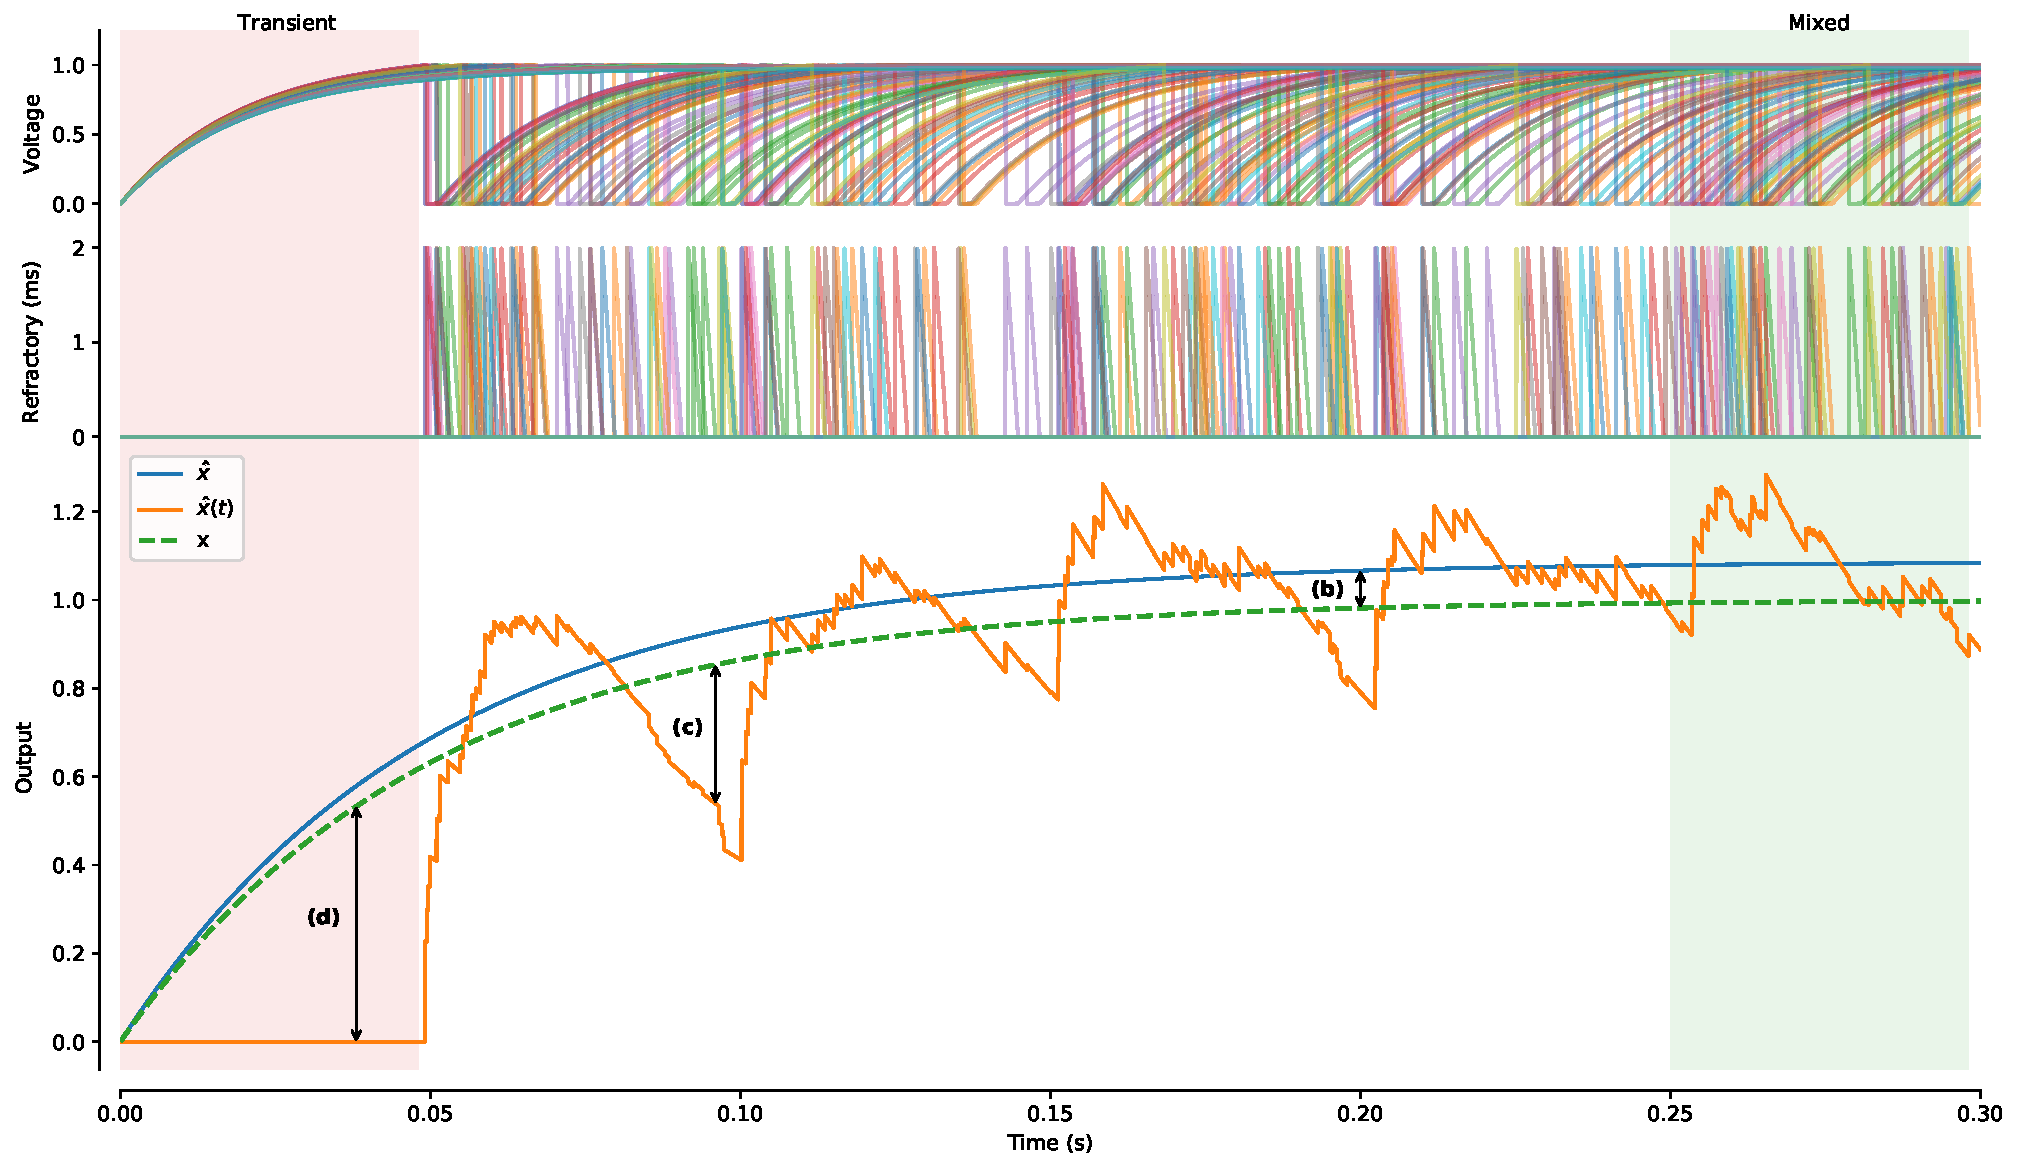
\includegraphics[width=\linewidth]{nef-error-types-a}
    \caption{Example Network Simulation}
    \label{fig:nef-error-types-a}
  \end{subfigure}
  \begin{subfigure}[t]{.33\textwidth}
    \centering
    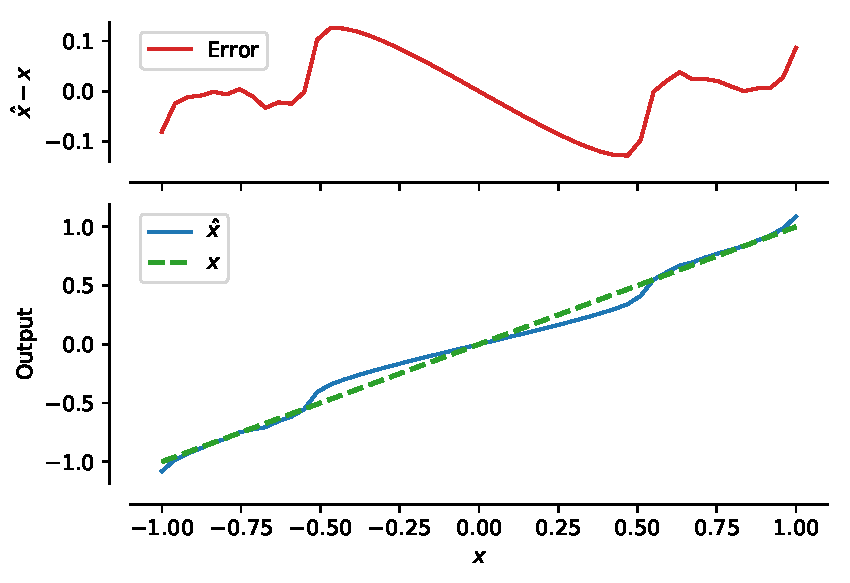
\includegraphics[width=\linewidth]{nef-error-types-b}
    \caption{Static Distortion}
    \label{fig:nef-error-types-b}
  \end{subfigure}%
  \begin{subfigure}[t]{.33\textwidth}
    \centering
    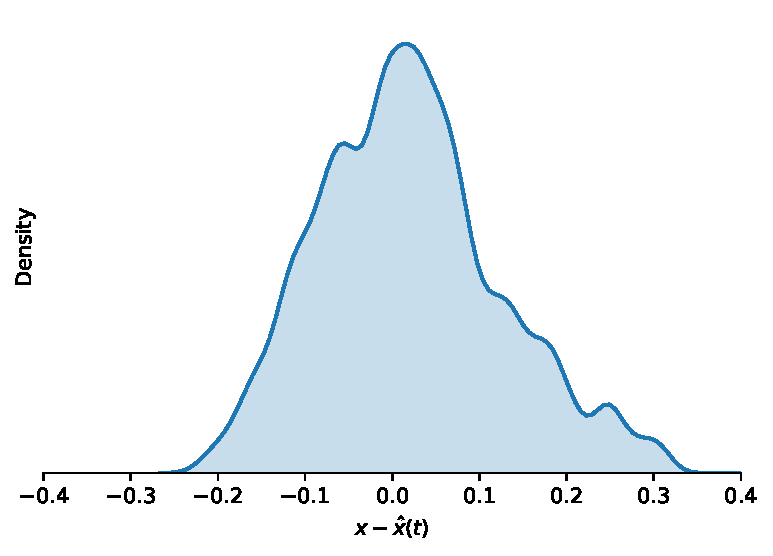
\includegraphics[width=\linewidth]{nef-error-types-c}
    \caption{Spiking Noise ($t > 0.15$\,s)}
    \label{fig:nef-error-types-c}
  \end{subfigure}%
  \begin{subfigure}[t]{.33\textwidth}
    \centering
    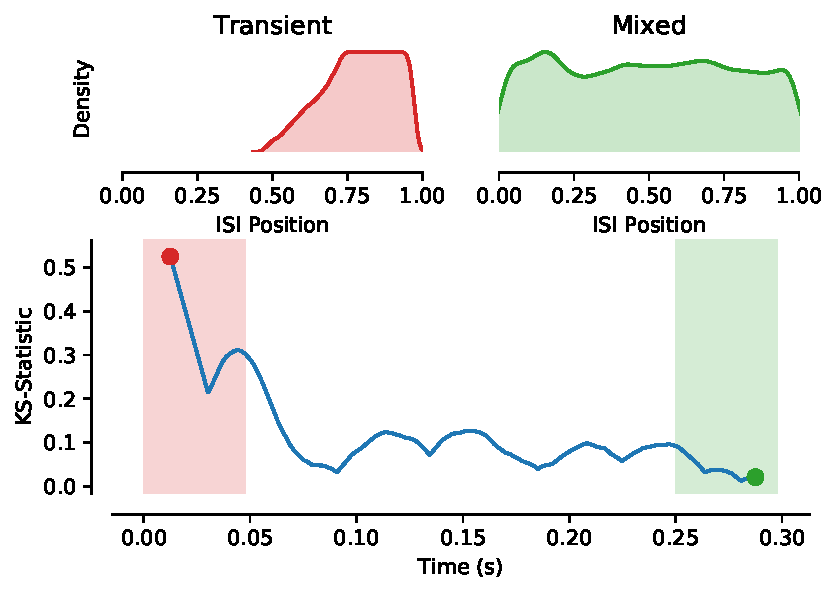
\includegraphics[width=\linewidth]{nef-error-types-d}
    \caption{State Discrepancy}
    \label{fig:nef-error-types-d}
  \end{subfigure}
  \caption[Three sources of error in spiking networks.]{ \label{fig:nef-error-types}
    Visualizing the three sources of error in a standard NEF network.
    (a)~A single simulation with arrows pointing to each type of error (b, c, d).
    (b)~Static distortion describes the difference between the linear combination of rate models and the desired static function.
    (c)~Spiking noise describes the difference between the spiking model and rate model.
    (d)~State discrepancy provides an instantaneous statistic capturing the difference between the spiking noise and a true Gaussian distribution ($p$-values~$< \numprint{e-6}$).
    See text for details.
  }
\end{figure}


\subsubsection{Static distortion}

The optimization problem described by equation~\ref{eq:decoder_solution} can be understood as fitting $n$ non-orthogonal static basis functions, $r_i$, to some desired static function, $f$~\citep{broomhead1988radial}.
Assuming relatively weak conditions on each $r_i$, namely monotonicity and continuity, any continuous $f$ may be approximated arbitrarily well by a linear combination of these basis functions~\citep{hornik1989multilayer}, as in equation~\ref{eq:trans-decode}.

Specifically, for a given $f$, a linear increase in the number of basis functions will reduce the root-mean-squared error~(RMSE) of the fit by the same factor.
This particular RMSE is named \emph{static distortion}, since it corresponds to the difference between the two static (i.e.,~non-temporal) functions.
We commonly refer to the RMSE as simply the ``error'' throughout,\footnote{%
\citet{eliasmith2003a} use ``error'' to refer to mean-squared error~(MSE), rather than the RMSE. This may lead to confusion when comparing across sources.}
and define ``precision'' to be the reciprocal of error.
Thus we say that the precision of a non-spiking network scales as $\bigoh{n}$.

Figure~\ref{fig:nef-error-types}~(b) visualizes the static distortion in two different ways.
The bottom plot, $x$ versus $\hat{x}$, compares the ideal against the approximation, and includes the dashed line $x = x$ for reference.
The upper plot, $x$ versus $\hat{x} - x$, provides a closer look to demonstrate that the error is continuous and with a mean close to zero.
The root-mean-squared value of the latter curve is the static distortion.

\subsubsection{Spiking noise}

By separating out the static distortion and looking at the difference $\transpose{\V{d}}a - \hat{x}$, we can isolate the role of equation~\ref{eq:rate-approximation} in the approximation error.
This is the difference between the spiking and non-spiking estimates, using the same set of basis functions.
We refer to this as the \emph{spiking noise}, since it corresponds to the variability in the estimate that is introduced by filtered spikes.

The variability in spike-trains across the population leads to an additional error term that scales as $\left( \tau \sqrt{n} \right)^{-1}$.
The $\tau^{-1}$ term comes from the variance of the filter's impulse response -- supposing equation~\ref{eq:lowpass-impulse} is applied to both the decoded spikes and the encoded input.
The $\sqrt{n}^{-1}$ term follows from the convergence rate of the central limit theorem~\citep[CLT;][]{berry1941accuracy, esseen1942liapunov}, and assuming the spiking noise is Gaussian and independent.
Under these assumptions, the spike noise asymptotically dominates the static distortion, and the SNN's feed-forward precision scales as $\bigoh{\tau \sqrt{n}}$.
However, in the context of Principle 3, the transformations of the signals are scaled by $\tau \theta^{-1}$, where $\theta$ is the time-constant of integration for the desired dynamical system, which results in a cancellation and the recurrent SNN having precision that scales as $\bigoh{\theta \sqrt{n}}$.

Figure~\ref{fig:nef-error-types}~(c) visualizes a kernel density estimate~\citep[KDE;][]{michael_waskom_2015_19108} of this error ($t > 0.15$\,s).
A Kolmogorov-Smirnov~(KS) test of $\transpose{\V{d}}a - \hat{x}$, versus a zero-mean Gaussian distribution with equal variance, produces a KS-statistic of $\approx 0.034$ ($p$-value~$< \numprint{e-6}$).
The KS-statistic is defined as the maximal discrepancy between the empirical cumulative density function~(CDF) and the model CDF~\citep[i.e.,~the supremum of their absolute difference;][]{massey1951kolmogorov}.
In this case, the distribution of spike noise is at most $3.4$\% different from a true Gaussian distribution.
This justifies the usage of the white noise term $\eta$ in equation~\ref{eq:decoder_solution}, since it captures $\approx 96.6$\% of the statistical variance between the filtered and decoded spiking and non-spiking models.
But why is there a difference?
In theory it should approach $0$ for sufficiently many samples, due to the CLT, but unfortunately it does not; there is a remaining systematic bias that never scales away (also see Figure~\ref{fig:poisson-neuron-scaling}).
It turns out that our assumption of independent Gaussian noise was not entirely correct -- an oversight that we will rectify at the end of this section.
But first, this motivates the discovery of a third and final source of error, that we now describe and analyze in detail.

\subsubsection{State discrepancy}

Intuitively, unbiased variability in spike-trains is achieved by all of the neurons being independently and uniformly \emph{ready to spike}.
Looking at the ``transient'' portion ($t < 0.05$\,s) of Figure~\ref{fig:nef-error-types}~(a), we see that all of the neurons are initially at rest, and thus physically cannot spike in time to keep up with the target.
This results in a period of time in which the error is quite large.
The error is overall the smallest towards the end of the simulation, at which point we say the neural states have ``mixed'' together.
We formalize these ideas by appealing to the inter-spike interval~(ISI) in a manner that will turn out to be quite important.

We define a neuron's relative ``ISI position''~(ISIP), $g_i$, to be its normalized position within the inter-spike interval that corresponds to the instantaneous firing rate of the ideal rate model.
For this, we fix our analysis at \emph{any given moment in time} and determine the next spike time.
To give an example, consider the LIF neuron's current state (although this same approach extends more generally to other neuron models) to have a voltage of $v_i$, remaining refractory period of $0 \le \rho_i \le \tau_\text{ref}$, input current of $s_i$, and a corresponding instantaneous target rate of $r_i$.
In the same way that we derived the rate model of the LIF neuron~(see derivation leading to equation~\ref{eq:lif-rate}), we may derive the neuron's ISIP according to how far along it is within the ideal ISI normalized by its length, $r_i^{-1}$:\footnote{%
If $r_i = 0$ then the neuron will not be active (and does not need to be), and so we can simply ignore it; the discussion, analysis, and results do not change.}
\begin{equation} \label{eq:lif-isip}
\begin{aligned}
g_i(v_i, \rho_i) &= 1 - \left( \rho_i + \tau_\text{RC} \ln \left( 1 + \frac{1 - v_i}{s_i - 1} \right) \right) r_i \\
% &= 1 - \frac{\rho_i + \tau_\text{RC} \ln \left( 1 + \frac{1 - v_i}{s_i - 1} \right)}{\tau_\text{ref} -\tau_\text{RC} \ln \left( 1 - \frac{1}{s_i} \right)} \text{.}
&= 1 - \frac{\rho_i + \tau_\text{RC} \ln \left( 1 + \frac{1 - v_i}{s_i - 1} \right)}{\tau_\text{ref} + \tau_\text{RC} \ln \left( 1 + \frac{1}{s_i - 1} \right)} \text{.}
\end{aligned}
\end{equation}
For example, $g_i(0, \tau_\text{ref}) = 0$, since the neuron is at the very beginning of its ISI.
Likewise, $g_i(1, 0) = 1$, as it has just spiked.

\begin{definition} \label{def:state-discrepancy}
The \emph{state discrepancy}, at some chosen moment in time, is the KS-statistic between the empirical ISIP distribution across the population, $\{g_i \, : \, i = 1 \ldots n\}$, and a true uniform distribution, $\mathcal{U}[0, 1]$.
\end{definition}

In Figure~\ref{fig:nef-error-types}~(d), we measure this value empirically across all of neurons, and at each time-step in the simulation, using a centered window of width $25$\,ms to smooth the estimate.
We see that the magnitude of the KS-statistic corresponds very closely to the error between the ideal and the spiking solution.
Although here we are looking at just a constant input for ease of visualization, we find that this statistic correlates highly (Pearson correlation coefficient $R = 0.90$, $p$-value~$< \numprint{e-6}$) with the spiking noise across a wide range of input frequencies (see Figure~\ref{fig:frequency-ks-test}).
This is surprising since the definition of state discrepancy does not invoke any usage of decoders, spikes, or filters in its construction; it merely describes how different the distribution of relative ISI positions are from that of a uniform distribution.

We now prove that our definition of state discrepancy is indeed the correct one, and in doing so provide a sufficient criteria for scaling away this source of error.
Specifically, this remaining source of error---state discrepancy---is tamed by minimizing the difference (KS-statistic) between a uniform distribution and the actual neuron's ``readiness to spike,'' as characterized by its ISIP~(e.g.,~equation~\ref{eq:lif-isip} for the case of a LIF model).

\vspace{1em}

\begin{theorem}[Scaling of feed-forward precision in the Neural Engineering Framework]
\label{thm:correctness}
Let $\V{\mu}(t) = \sum_{i=1}^n \left(a_i \ast h \right)(t) \V{d}^\V{f}_i- \sum_{i=1}^n \left( r_i(\V{x}) \ast h \right)(t) \V{d}^\V{f}_i$
% \transpose{\V{d}}a - \hat{x}$
be the spiking noise.
If the ISIPs, $g_i$, are uniformly and independently distributed, then:
\begin{enumerate}
\item $\expect{ \V{\mu}(t) } = 0$; hence the expected spike noise is exactly zero at all times (no systematic bias), 
\item $\sqrt{\variance{\V{\mu}(t)}} = \bigoh{\left(\tau \sqrt{n}\right)^{-1}}$ is the standard error, or root-mean-squared error; hence the precision scales as $\bigoh{ \tau \sqrt{n} }$ at all times.
% \item equation~\ref{eq:rate-approximation} has residual error with the statistic $\V{\mu}(\cdot) \sim \mathcal{N}\left(0, \sigma^2 \right)$, where $\sigma = \bigoh{ \left( \tau \sqrt{n} \right)^{-1} }$.
\end{enumerate}
\end{theorem}
We prove each statement, in order, after a few remarks.
We prove something slightly more general, and without invoking asymptotics until the very end.
We also do so without assuming any particular neuron model -- only that it has a well-defined ISIP.
We shift our frame of reference, without loss of generality, such that we are currently observing $t = 0$.
We then forecast the system out into the future, assuming the representation is held constant.
But this does not make any assertions about the causal dynamics of the representation.
This is because the statements in this theorem are only interested in the distribution of a statistic at arbitrarily small values of $t \rightarrow 0^+$ with respect to the shifted time frame.
% $t = \epsilon$ in the one-sided limit of $\lim_{\epsilon \rightarrow 0^+} \eta(t)$.
Hence, our work provides a more general result than what is needed.
In order to give a concrete result, we suppose the synapse model is equation~\ref{eq:lowpass-impulse}, but this is not a hard requirement.
Likewise, we initialize the synapses to $0$, without loss of generality by linearity.
To remove boilerplate in the notation we substitute $r_i \leftarrow r_i(\V{x}(t))$.
We have verified each of the following equations with numerical experiments~(not shown).

\subsubsection{Preliminaries}

Let $\tilde{y}_i(t; t_i) = \left(a_i \ast h \right)(t)$ be the fast-forward simulation of the $i^\text{th}$ neuron up to time $t \ge 0$, supposing $t_i = \left(1 - g_i\right)r_i^{-1}$ is the next spike-time ($0 \le t_i \le r_i^{-1}$) by our definition of the ISIP.
% The initial state of the synapse is some constant, that we assume to be zero without loss of generality.
Let $T_i$ be the random variable whose realizations are $t_i$.
Hence, $T_i \sim \mathcal{U} [ 0, r_i^{-1} ]$,
with a probability density function~(PDF) and cumulative density function~(CDF) described by:
\begin{equation} \label{eq:spike-distribution}
f_{T_i}(t_i) = r_i \quad \iff \quad P(T_i \le t_i) = t_i r_i \text{.}
\end{equation}
By enumerating over the spike-times, we have:
\begin{align*}
\tilde{y}_i(t; t_i) &= \sum_{0 \le j \le r_i \cdot (t - t_i)} (\delta_{j / r_i + t_i} \ast h)(t) \\
&= \sum_{0 \le j \le r_i \cdot (t - t_i)} \frac{1}{\tau} e^{-\frac{t - (j/r_i + t_i)}{\tau}} \\
&= \sum_{0 \le j \le r_i \cdot (t - t_i)} \frac{1}{\tau} \left( \underbrace{e^{-\left(r_i \tau\right)^{-1}}}_{c_i} \right)^{r_i \cdot (t - t_i) -j}  \text{,}
\end{align*}
where $0 < c_i < 1$ is an important constant that we remark is dimensionless (i.e.,~unitless), and also time-invariant (i.e.,~depends only on $r_i$ and $\tau$).
We then re-arrange as follows:
\begin{align}
\label{eq:neuron}
\implies \quad \tilde{y}_i(t; t_i) &= \frac{c_i^{r_i \cdot (t - t_i) + 1}}{\tau} \sum_{1 \le j \le r_i \cdot (t - t_i) + 1} \left( c_i^{-1} \right)^j \quad \text{(note: altered index)} \nonumber \\
&= \frac{c_i^{r_i \cdot (t - t_i) + 1}}{\tau} \left( \frac{1}{c_i} \right) \frac{\left( \frac{1}{c_i} \right)^{\floor{r_i \cdot (t - t_i) + 1}} - 1}{\frac{1}{c_i} - 1} \quad \text{(geometric series)} \nonumber \\
&\,= \frac{c_i^{e_i(t; t_i)} - c_i^{r_i \cdot (t - t_i) + 1}}{\tau(1 - c_i)}
\end{align}
where:
\begin{equation}
\begin{gathered}
\label{eq:delta} %(r_i \cdot (t - t_i) + 1) - \floor{r_i \cdot (t - t_i) + 1} 
e_i(t; t_i) = r_i \cdot (t - t_i) - \floor{r_i \cdot (t - t_i)} \\
0 \le e_i(t; t_i) < 1 \text{,}
\end{gathered}
\end{equation}
is a type of truncation error.
Equation~\ref{eq:neuron} provides a closed-form solution for $\tilde{y}_i$.
In addition, the lower/upper bounds of $e_i(t; t_i)$ supply its upper- and lower-envelopes, respectively:
\begin{equation*}
\frac{c_i - c_i^{r_i \cdot (t - t_i) + 1}}{\tau(1 - c_i)} < \tilde{y}_i(t; t_i) \le \frac{1 - c_i^{r_i \cdot (t - t_i) + 1}}{\tau(1 - c_i)} \text{.}
\end{equation*}

Now, the analysis proceeds in the following manner.
We pick our $t$, and then sample our $t_i$.
This determines $e_i(t; t_i)$ for each neuron, by a cyclic rotation $r_i t_i$ (modulo $1$) from equation~\ref{eq:delta}.
We then define a new random variable $\tilde{Y}_i(t) = \tilde{y}_i(t; T_i)$, which one can understand as being distributed by ``mapping'' the random variable $T_i$ through the function $\tilde{y}_i$ for some chosen $t$.
Realizations of this random variable correspond directly to $\left(a_i \ast h \right)(t)$ by construction. 
% As an aside, for the special case of uniform $T_i$, the mapping $\tilde{y}_i$ actually corresponds to a cyclically shifted version of the inverse CDF of $\tilde{Y}_i(t)$\footnote{This requires a subtle monotonicity argument. The CDF of $\tilde{Y}_i$ can therefore be derived by inverting the unshifted $\tilde{y}_i$, but the result is not very nice to work with due to some discontinuities in its derivative.}.
%\begin{align}
%\label{eq:z}
%z_i(t_i; t) := \tilde{y}_i(t; t_i)
%\end{align}
%to view $Z_i(t)$ as a random variable that is obtained by ``mapping'' the distribution of $T_i$ through the function $\tilde{y}_i$ for some chosen $t$.  

% Then the random variable $\V{\tilde{X}}(t) := \sum_i \V{d}_i \tilde{Y}_i(t)$ is the decoded estimate obtained by forming a mixture of $\tilde{Y}_i(t)$. The following subsections will analyze the expectation and variance of each $\tilde{Y}_i(t)$ to determine the expected error and variability at time $t$.

\subsubsection{Proof of zero-mean error}

We apply the law of the unconscious statistician~(LOTUS) to $\tilde{Y}_i(t)$:
\begin{align}
\label{eq:a_expectation}
\expect{\tilde{Y}_i(t)} &= \int_D \tilde{y}_i(t; t_i) f_{T_i}(t_i) \,dt_i, \quad \text{where $D$ is the domain of $T_i$} \nonumber\\
          &= \int_D \frac{c_i^{e_i(t; t_i)} - c_i^{r_i \cdot (t - t_i) + 1}}{\tau(1 - c_i)} f_{T_i}(t_i) \,dt_i, \quad \text{by equation~\ref{eq:neuron}} \nonumber\\
          &= \frac{1}{\tau(1 - c_i)} \left( \int_0^{1} c_i^{e_i(t; t_i)} \,de_i(t; t_i) - \int_0^{r_i^{-1}} c_i^{r_i \cdot (t - t_i) + 1} (r_i) \,dt_i \right) \nonumber\\
          &= \frac{1}{\tau(1 - c_i)} \left( (-r_i \tau) e^{-e_i(t; t_i)/(r_i \tau)} \bigg|_{e_i(t; t_i) = 0}^{1} - (r_i \tau) c_i^{r_i \cdot (t - t_i) + 1} \bigg|_{t_i = 0}^{r_i^{-1}} \right) \nonumber\\
          &= \frac{r_i}{(1 - c_i)} \left(  (1 - c_i) - \left( c_i^{r_i t} - c_i^{r_i t + 1} \right)  \right) \nonumber\\
          &= r_i \cdot (1 - e^{-t/\tau}) \text{.}
\end{align}
Therefore, by linearity of expectation, the expected error at time $t$ is:
\begin{equation}
\begin{aligned}
\expect{\V{\mu}(t)} &= \expect{\sum_{i=1}^n \left(a_i \ast h \right)(t) \V{d}^\V{f}_i - \sum_{i=1}^n \left( r_i \ast h \right)(t) \V{d}^\V{f}_i } \\
&= \sum_{i=1}^n r_i \cdot (1 - e^{-t/\tau}) \V{d}^\V{f}_i - \sum_{i=1}^n \left( r_i \ast h \right)(t) \V{d}^\V{f}_i \\
&= 0 \text{.}
\end{aligned}
\end{equation}
This completes our proof of the first statement. $\hfill \qed$

Note that we have not needed to use our assumption about the independence of samples.
However, to obtain a closed-form solution for the variance, we will need to assume that $g_i$, and thus $t_i$, are independently sampled (i.e.,~the voltage vectors and refractory periods are not coupled with one another across time), as is the case for typical NEF networks.
\citet{boerlin2013predictive} have shown that if the neural states do have a mechanism for collaborating in a global manner, then they can synchronize their activity; this corresponds to a means of \emph{dependent} sampling that reduces the following variance.

\subsubsection{Proof of spiking variance}

To compute $\variance{\tilde{Y}_i(t)} = \expect{\tilde{Y}_i(t)^2} - \expect{\tilde{Y}_i(t)}^2$ we rewrite the second moment:
\begin{align*}
\expect{\tilde{Y}_i(t)^2} &= \expect{\left( \frac{c_i^{e_i(t; T_i)} - c_i^{r_i \cdot (t - T_i) + 1}}{\tau(1 - c_i)} \right)^2} \\
&= \left( \frac{1}{\tau(1 - c_i)} \right)^2 \left( \expect{\left(c_i^{e_i(t; T_i)}\right)^2 } - 2 \expect{c_i^{e_i(t; T_i) + r_i \cdot (t - T_i) + 1}} + \expect{\left( c_i^{r_i \cdot (t - T_i) + 1} \right)^2} \right)
\end{align*}
and then separately determine each expectation.
The PDFs of $c_i^{e_i(t; T_i)}$ and $c_i^{r_i \cdot (t - T_i) + 1}$ are both $r_i \tau / x$ over their respective domains. This can be seen directly:
\begin{align*}
\frac{\partial}{\partial x} P \left( c_i^{e_i(t; T_i)} \le x \right) &= \frac{\partial}{\partial x} P \left( e_i(t; T_i) \ge -r_i \tau \ln x \right) \\
&= \frac{\partial}{\partial x} \left( 1 - (-r_i \tau \ln x) \right) \\
&= r_i \tau / x .
\end{align*}
and the proof for $c_i^{r_i \cdot (t - T_i) + 1}$ is analogous.
As an aside, these two facts can be used to give a slightly different derivation for equation~\ref{eq:a_expectation}.
Applying LOTUS to each of these random variables gives:
\begin{align*}
\expect{\left(c_i^{e_i(t; T_i)}\right)^2} &= \int_{c_i}^1 \frac{r_i \tau}{x} x^2 \,dx = \frac{r_i \tau x^2}{2} \bigg|_{x = c_i}^1 = \frac{r_i \tau \left(1 - c_i^2 \right)}{2} \\
\expect{\left(c_i^{r_i \cdot (t - T_i) + 1}\right)^2} &= \int_{c_i^{r_i t + 1}}^{c_i^{r_i t}} \frac{r_i \tau}{x} x^2 \,dx = \frac{r_i \tau x^2}{2} \bigg|_{x = c_i^{r_i t + 1}}^{c_i^{r_i t}} = \frac{r_i \tau \left(1 - c_i^2 \right) c_i^{2 r_i t}}{2} .
\end{align*}
To compute the remaining expectation, we require further insight into $e_i(t; T_i) = r_i \cdot (t - t_i) - \floor{r_i \cdot (t - t_i)}$.
Define $k_i(t) = \floor{r_i t}$ as the spike index of $t$.  %Then the $i^{th}$ neuron has spiked $k_i(t - t_i) + 1 = \floor{r_i \cdot (t - t_i) + 1}$ times at time $t$. More importantly, 
Recall that $t$ is fixed in this discussion.
The congruence relation \mbox{$t_i = t - k_i(t)/r_i \equiv t \ (\text{mod}\ r_i^{-1})$} is also a discontinuity in $e_i(t; t_i)$ with respect to $t_i$; that is when the spike becomes aligned with $t$ in the current interval.
Namely, if $0 \le t_i \le t - k_i(t)/r_i$, then $\floor{r_i \cdot (t - t_i) + 1} = \floor{k_i(t) + 1} = k_i(t) + 1$. Likewise, if $t - k_i(t)/r_i < t_i \le r_i^{-1}$, then $\floor{r_i \cdot (t - t_i) + 1} = k_i(t)$.
We now apply LOTUS once more, along with the above facts to split up the integral.
\begin{align*}
\expect{ c_i^{e_i(t; T_i) + r_i \cdot (t - T_i) + 1} } &= \int_0^{r_i^{-1}} c_i^{2(r_i \cdot (t - t_i) + 1) - \floor{r_i \cdot (t - t_i) + 1}} (r_i) \, dt_i \\
&= r_i \left( \int_0^{t - k_i(t)/r_i} c_i ^ {(2r_i t - k_i(t) + 1) - (2r_i t_i)} \, dt_i + \int_{t - k_i(t)/r_i}^{r_i^{-1}} c_i^{(2r_i t - k_i(t) + 2) - (2r_i t_i)} \, dt_i \right) \\
&= r_i c_i^{2r_i t - k_i(t) + 1} (\tau / 2) \left( e^{2t_i / \tau} \bigg|_{t_i=0}^{t - k_i(t)/r_i} + c_i e^{2t_i / \tau} \bigg|_{t_i=t - k_i(t)/r_i}^{r_i^{-1}} \right) \\
&= r_i c_i^{2r_i t - k_i(t) + 1} (\tau / 2) \left( c_i^{-2 r_i \cdot (t - k_i(t)/r_i)} - 1 + c_i^{-1} - c_i^{-2r_i \cdot (t - k_i(t)/r_i) + 1} \right) \\
&= r_i \tau (1 - c_i) \left(c_i^{k_i(t) + 1} + c_i^{2r_i t - k_i(t)} \right) / 2
\end{align*}
Substituting all of these expectations into the initial formula yields:
\begin{align*}
\variance{\tilde{Y}_i(t)} = r_i \left( \frac{\left(1 - c_i^2 \right)\left(1 + c_i^{2r_i t}\right)}{2\tau \left(1 - c_i \right)^2} - \frac{\left( c_i^{k_i(t) + 1} + c_i^{2r_i t - k_i(t)} \right)}{\tau(1 - c_i)} - r_i \cdot \left(1 - c_i^{r_i t} \right)^2 \right) 
\end{align*}
Asymptotic analysis reveals that this scales as $\bigoh{\tau^{-2}}$ as $\tau \rightarrow 0^+$.
As well, we use the fact that regularized least-squares finds
$\V{d}_i^\V{f}$ that are independently distributed according to $\mathcal{N}(0, \sigma^2)$ where $\sigma = \bigoh{n^{-1}}$ -- i.e., variance scales as $\bigoh{n^{-2}}$.
Finally we use equation~\ref{eq:a_expectation} in the second step below, and then leverage the property that for any two uncorrelated \emph{zero-mean} variables, $A$ and $B$, we have $\variance{AB} = \variance{A}\variance{B}$.
Therefore,
\begin{align*}
\sqrt{ \variance{ \V{\mu}(t) } } &= \sqrt{ \variance{\sum_{i=1}^n \left(a_i \ast h \right)(t) \V{d}^\V{f}_i- \sum_{i=1}^n \left( r_i \ast h \right)(t) \V{d}^\V{f}_i} } \\
&= \sqrt{ \variance{\sum_{i=1}^n \left( \tilde{Y}_i(t) - \expect{ \tilde{Y}_i(t) } \right) \V{d}^\V{f}_i } } \\
&= \sqrt{ n \variance{\tilde{Y}_\cdot(t)} \variance{\V{d}^\V{f}_\cdot}} \\
&= \sqrt{ n \bigoh{ \tau^{-2} } \bigoh{ n^{-2} } } \\
&= \bigoh{ \frac{1}{\tau \sqrt{n}} } \text{.} &\pushright{\qed}
\end{align*}

\subsubsection{Satisfying the uniform ISIP criteria}

Theorem~\ref{thm:correctness} has important consequences for the correctness of NEF networks and the precision of neural computation in general.
Assuming neural states remain distributed in a manner that satisfies the criteria of uniform ISIPs, then equation~\ref{eq:rate-approximation}, which forms the basis for the efficient training of NEF networks, is mathematically correct.
Thus, precision continues to scale (i.e.,~error converges to zero by the CLT), even as:
(1)~the number of neurons goes towards infinity~(see Figure~\ref{fig:poisson-neuron-scaling}), and
(2)~for arbitrarily high-frequency stimuli~(see Figure~\ref{fig:poisson-frequency-scaling}).
This ensures that the NEF, and its postsynaptic current coding scheme (see section~\ref{sec:psc-coding}), is asymptotically correct -- even when encoding arbitrarily high-frequency signals into spikes with arbitrarily small synaptic time-constants and low firing rates.
We summarize many of these scaling properties in section~\ref{sec:scalability}.

\fig{frequency-ks-test}{1}{Linear correlation between neural states and error.}{
  Relationship between state discrepancy~(KS-statistic; definition~\ref{def:state-discrepancy}) and representational error induced by filtered spikes~(RMSE), for sinusoidal stimuli of varying frequencies.
  (Left)~Empirical distribution of ISI positions (equation~\ref{eq:lif-isip}) is compared to the ideal uniform distribution using the KS-statistic ($p$-values~$< \numprint{e-6}$).
  % In the ideal case, the spiking LIF model is equal to its non-spiking counterpart in the sense of expectation.
  (Right)~The RMSE is highly correlated with the KS-statistic, with a Pearson correlation coefficient of $R = 0.90$ ($p$-value~$< \numprint{e-6}$).
}

However, in the NEF, when using LIF neurons, this criteria is violated as the frequency of the represented signal increases.
To demonstrate, Figure~\ref{fig:frequency-ks-test} simulates a communication channel ($n = \numprint{2500}$, $\dt{} = 0.1$\,ms, $\tau = 1.6$\,ms, $\tau_\text{RC} = 20$\,ms, $\tau_\text{ref} = 2$\,ms), with tuning curves uniformly distributed to achieve maximum firing rates of $50$--$100$\,Hz, in order to encode sinusoid stimuli of increasing frequencies (visualizing 95\% confidence interval, bootstrapped across 5 random configurations at each frequency).
For $0$\,Hz (constant) inputs, the ISIP distribution is uniform (KS-statistic~$<0.0002$), as we should expect (i.e.,~the neural states remain independently mixed for a constant input).
% This verifies the numerics of our spiking LIF implementation\TODO{cite Nengo LIF improvements}, as we should expect that a constant input causes each neuron to spend an equal amount of time at each position within its ideal ISI.
However, as the frequency increases, so does the state discrepancy (see left).
Likewise, the state discrepancy is highly correlated ($R = 0.90$) with the RMSE of the spike noise (see right).
Even though the state discrepancy is $< 6$\% for input frequencies up to $100$\,Hz, it is important to remind the reader that this is a systematic error that \emph{does not scale away} with higher neuron counts.
On the one hand this makes theoretical predictions regarding the information-processing capabilities of LIF neurons for stimuli with various statistics, and in particular suggests a nonlinear transfer function that may have some functional relevance -- but, on the other hand, here we are interested in understanding how this formalism relates to minimizing error and maximizing information throughput.

In order to scale away the state discrepancy, we note that the uniform ISIP assumption may be satisfied in a number of ways, many of which are validated in
section~\ref{sec:poisson-spiking}:
\begin{enumerate}
\item The state of the system is initialized such that $g_i$ is uniform.
For the case of the LIF model, one can invert equation~\ref{eq:lif-isip} and solve for $(v_i, \rho_i)$ from a uniform sample, and then use this to initialize the state of each neuron.
We do so in many of our experiments (including Figure~\ref{fig:frequency-ks-test}) in order to remove the initial transient that would otherwise be a statistical anomaly~(see Figure~\ref{fig:nef-error-types}~(d)).
Given a constant representation, the neural states naturally remain mixed due to heterogeneity in the encoding.
However, this does not guarantee invariance over time for time-varying stimuli; leakage in the model as well as rapid inhibition can skew the ISIPs back towards zero.

\item The neuron model is replaced by a spiking rectified linear (ReLU) unit, also known as a (non-leaky) integrate-and-fire neuron. This model rectifies its input current, such that its state only evolves in one direction.
This can also be achieved by setting $\tau_\text{RC}$ to be sufficiently large and lowering the neuron's voltage floor, as in \citet{boerlin2013predictive}.
Incidentally, \citet[][pp.~238--239]{eliasmith2003a} discovered that an integrator's performance was improved by increasing $\tau_\text{RC}$, but attributed this improvement to static distortion being minimized by linear tuning curves, instead of having reduced the overall state discrepancy~\citep[also see][appendix~F.1]{eliasmith2003a}.

\item Noise is introduced to the neuron model, to maintain a uniform subthreshold state~\citep[][pp.~132--133]{eliasmith2003a}.
Indeed, this is the same assumption made by \citet[][p.~134]{eliasmith2003a} in their assessment of the quality of spiking neural representation.

\item The neuron model is replaced by its Poisson-spiking counterpart; that is, \emph{any} static nonlinearity supplied to a Poisson spike-generator.
Due to the memoryless nature of the Poisson process, at any given moment in time, the model is always uniformly ready to spike with the ideal probability (see section~\ref{sec:poisson-spiking}).

\end{enumerate}
Future work is required for more biologically-detailed neuron models and synapses.
We conjecture that the role of many adaptive mechanisms in biological systems is to invariantly maintain the uniform ISIP criteria with respect to the time-varying statistics of the represented signal.
Such mechanisms would facilitate efficient coding by maximizing information throughput for a fixed energy-budget (see section~\ref{sec:energy-minimization} and \citet[][pp.~127,~Table~4.1]{eliasmith2003a}).

\subsection{Scalability}
\label{sec:scalability}

In this section we summarize the general trade-offs associated with scaling NEF networks.
Some application-specific trade-offs are discussed in section~\ref{sec:delay-applications}.

\begin{sidewaystable}
\centering
  \begin{tabular}{@{}llll@{}} \toprule
    Property & Scaling & Context & References \\
    \midrule
    Multiply-adds per step & $\bigoh{nq}$ & Inference & \citet{voelker2018} \\
    Total memory & $\bigoh{nq}$ & Inference & \citet{mundy2015, voelker2018} \\
    Time \& memory & $\bigoh{nq}$ & Training & section~\ref{sec:principle2} (assuming randomized SVD) \\
    Static precision & $\bigoh{n}$ & Fitting & section~\ref{sec:spike-coding} \\
    Spiking precision & $\bigoh{\tau \sqrt{n}}$ & Feed-forward & section~\ref{sec:spike-coding} \\
    Spiking precision & $\bigoh{\theta \sqrt{n}}$ & Recurrent & section~\ref{sec:spike-coding} \\
    Bandwidth (Hz) & $\bigoh{\left(2\pi \tau \right)^{-1}}$ & Fixed energy & section~\ref{sec:energy-minimization} \\
    Relative energy & $\bigoh{2\pi \tau f }$ & Fixed precision & section~\ref{sec:energy-minimization} \\
    Neuron count & $\bigoh{2 \pi f}$ & Fixed precision, $\tau = f^{-1}$ & equation~\ref{eq:psc-code-power} and Figure~\ref{fig:poisson-frequency-scaling} \\
    Dimensionality & $\bigoh{ n^{\frac{2}{3}} }$ & Fixed precision & \citet[][p.~60]{gosmann2018} \\ % this is actually big omega
    \bottomrule
  \end{tabular}
  \caption[Summary of scaling trade-offs in the NEF.]{ \label{tab:scalability}
    A summary of trade-offs present in standard NEF networks.
    Each property's scaling is context-dependent.
    Variables include neuron count ($n$), dimensionality ($q$), synaptic time-constant ($\tau$), system-level time-constant ($\theta$), and representational frequency ($f$).
    % Many of these are abusing big-oh notation and should be big-theta or big-omega...
  }
\end{sidewaystable}

Table~\ref{tab:scalability} provides a comprehensive list of all such trade-offs that we are aware of to date.
This includes guarantees on training time, resources for simulation, precision (in spiking, non-spiking, feed-forward, and recurrent architectures), energy usage, dimensionality, and finally relationships between signal bandwidth, synaptic time-constants, and neuron counts.
For the scaling of spiking networks, we assume that the uniform ISIP criteria of Theorem~\ref{thm:correctness} is satisfied.
References to relevant sections and literature are included in the right-hand column.

As a brief but important aside, the trade-offs that involve time do so by fixing some time-scale of interest.
That is, one chooses some unit associated with $\tau$ (e.g.,~seconds), or $f$ (e.g.,~Hertz), and so forth.
In theory, and in practice, the relative time-scales are what end up being important in determining the behaviour of the system.
% As every time-constant has some unit of time associated with it, their relation to one another is what determines the system's behaviour.
For example, if one were to slow down all of the time-constants in the network ($\tau$, $\tau_\text{RC}$, $\tau_\text{ref}$, $\dt{}$) by a factor of $10$, while increasing all of the rates in the network by the same factor, this would automatically be equivalent to speeding up the stimulus' frequency (reciprocal of time) by a factor of $10$ in the original network.
Nothing else needs to be changed in order to compress or expand our perspective of time; weights, neuron counts, and decoded quantities are all unitless.
This simply follows from dimensional analysis and consistent usage of time-constants and frequencies throughout, which highlights the importance of taking physical dimensions into consideration throughout each level of analysis.
In theory, this means these trade-offs can be applied to any time-scale, although in practice biological and hardware constraints often determine the relevant time-scales.

\newpage

\subsection{Completeness}
\label{sec:nef-turing}

Continuous-time dynamical systems, such as those implemented by the NEF, serve as powerful, \emph{universal models} of computation~\citep{bennett1995universal}.
For example, a dynamical system describing the motion of a particle in three-dimensional space, consisting of a finite number of equations, is capable of simulating a Turing machine~\citep{moore1990unpredictability}.
Such systems are physically implementable, while being undecidable in the sense that virtually every question about their long-term behaviour is impossible to predict, even with perfect knowledge~\citep[][]{moore1991generalized}.

As established in the previous sections, the NEF may be used to train a network to approximate any continuous-time dynamical system arbitrarily well, with precision scaling in the number of neurons.
Therefore, it follows that the class of NEF networks are equivalent in power to a Turing machine.
The same can be said for continuous-time RNNs and other SNN models~\citep{funahashi1993approximation, thalmeier2016learning}.
In theory, this means that these methods have the potential to implement arbitrary algorithms in distributed networks of computing elements.

In some ways, the universality of continuous-time dynamical computations should not come as a surprise, as 
a Turing machine is nothing more than a discrete-time dynamical system with an unbounded (but finite for decidable tasks) number of state-variables~\citep{turing1938computable}.
Early work by \citet{voelker2014controlling} provided a constructive proof of Turing-completeness in the NEF, by using the Semantic Pointer Architecture~\citep[SPA;][]{eliasmith2013build} to process the instructions of algorithms encoded into graphs that were sufficiently powerful to emulate multiple pushdown automata.
% However, we have since moved away from this line of work, towards developing a systematic understanding of leveraging neuromorphic models of computation towards NEF-based computations.

There is extensive literature on computability in both physical and non-physical substrates, leveraging dynamics that are either discrete or continuous in space and time.
However, these theoretical results do not have much to say in practice about the constraints that a certain task will impose on the system, the resources needed by an optimal solution, or likewise the algorithms that demand the least amount of power according to the physical devices leveraged by the model of computation.

We see these concerns as being in the realm of what should, and can, be addressed by frameworks, methods, and tools (e.g.,~NEF and~Nengo) that aim to expose and leverage some underlying model of computation.
Thus, we do not take Turing-completeness to be the ultimate arbiter of whether some model of computation is suitable for describing the brain.
Rather, we take this discussion as theoretical justification for the expressive power of dynamical systems, and therefore the utility in having well-understood tools for realizing them in neuromorphic hardware.
The following sections are concerned with the robustness and extensibility of these tools.

\subsection{Robustness}
\label{sec:nef-robustness}

Many different notions of robustness in the NEF have already been studied by \citet{eliasmith2003a}, \citet{eliasmith2012}, and \citet{eliasmith2013build}.
Robustness to sources of variability and modelling errors in particular are essentially built-in to the framework.
The NEF uses variable spikes to encode information, and heterogeneous basis functions for transformation, with zero-mean error (see Theorem~\ref{thm:correctness}).
This enables the network's function to remain robust to randomly dropped or delayed spikes, weights that are quantized, perturbed, or sparsified, the removal of neurons, intrinsic noise, and similar sources of variability.

But in addition, there is a distinctly different kind of robustness that, to our knowledge, has not been discussed in the literature.
As demonstrated in section~\ref{sec:chaos}, every non-trivial recurrent NEF network is naturally chaotic at the level of individual neurons.
Yet, in spite of this chaos, the network functions correctly at the level of its state-space representation.
Robustness to chaos has an important practical consequence: small measurement errors in the state of individual neurons---arising either from mechanisms in the system that rely on noisy observations, or through modelling errors of the mechanisms themselves---may be tamed at the population level. 
For example, an NEF integrator can be supplied a white noise process, of sufficiently small amplitude (relative to the radius of its stable point), and it will remain within the strange attractor corresponding to its fixed point, indefinitely. 
This enables a working memory that can persist states for long periods of time even in the presence of noise~\citep{singh2004}.

In contrast, the methods of \citet{boerlin2013predictive} are not robust to such noise models, since they treat any noise as being a part of the signal.
To be precise, if one constructs an integrator using their methods, and provides the same white noise process described above, then it will compute the exact integral of white noise: a random walk (not shown).
After a sufficient amount of time, the state of the system will have completely wandered off from where it had started, with no way of remembering the value that it was supposed to store.
This occurs even when the input is filtered using a lowpass synapse with an arbitrarily long time-constant; its integral is still a transient stochastic process.

We take this to be of importance in the context of biological modelling and neuromorphic hardware, since there is usually some undesirable signal, error, noise, or likewise, that must eventually be accounted for in some manner.
Integrating zero-mean error is not a general solution (although it may be sufficient in some contexts in conjunction with saturation effects).
The NEF accounts for this by explicitly incorporating a noise model into the training procedure (see equation~\ref{eq:decoder_solution}) and implicitly establishing an array of fixed points in state-space~\citep[][p.~237]{eliasmith2003a}.
In addition, the NEF is robust to the use of a number of different neuron models and synapse models, as is the focus of extensions discussed below.

\subsection{Extensibility}
\label{sec:nef-extensibility}

As stated in section~\ref{sec:neuromorphic}, NEF networks have been deployed on a number of different backends, including:
SpiNNaker~\citep{mundy2015},
Neurogrid~\citep{dethier2011brain},
Braindrop~\citep{braindrop2019},
Loihi~\citep{nengoloihi},
TrueNorth~\citep{fischl2018},
a VLSI prototype~\citep{corradi2014},
several FPGA implementations~\citep{naylor2013managing, wang2014compact, berzish2016, wang2017neuromorphic, nengofpga},
and several GPUs~\citep{bekolay2014, rasmussen2018nengodl, blouw2018a}.
This would not have been possible if not for the extensibility of the NEF -- that is, its flexibility in accounting for various non-idealities~\citep[e.g.,~][]{voelker2017iscas}.

Our work in this direction is the topic of chapter~\ref{chapt:nef-extensions}.
Of particular focus are the higher-order synapses with variable time-constants on Braindrop, and the configurably-delayed axons on Loihi.
Our extensions can successfully leverage both to improve network-level computation.
The focus of chapter~\ref{chapt:results} is then to showcase several recurrent SNNs deployed on both architectures, while using the same high-level model description for each network.
The machinery of the NEF and Nengo, together with the extensions in this thesis, take care of compiling the model description onto the hardware while respecting its constraints and leveraging its dynamical primitives~\citep{braindrop2019}.
